\section{Evaluation}
\begin{figure}
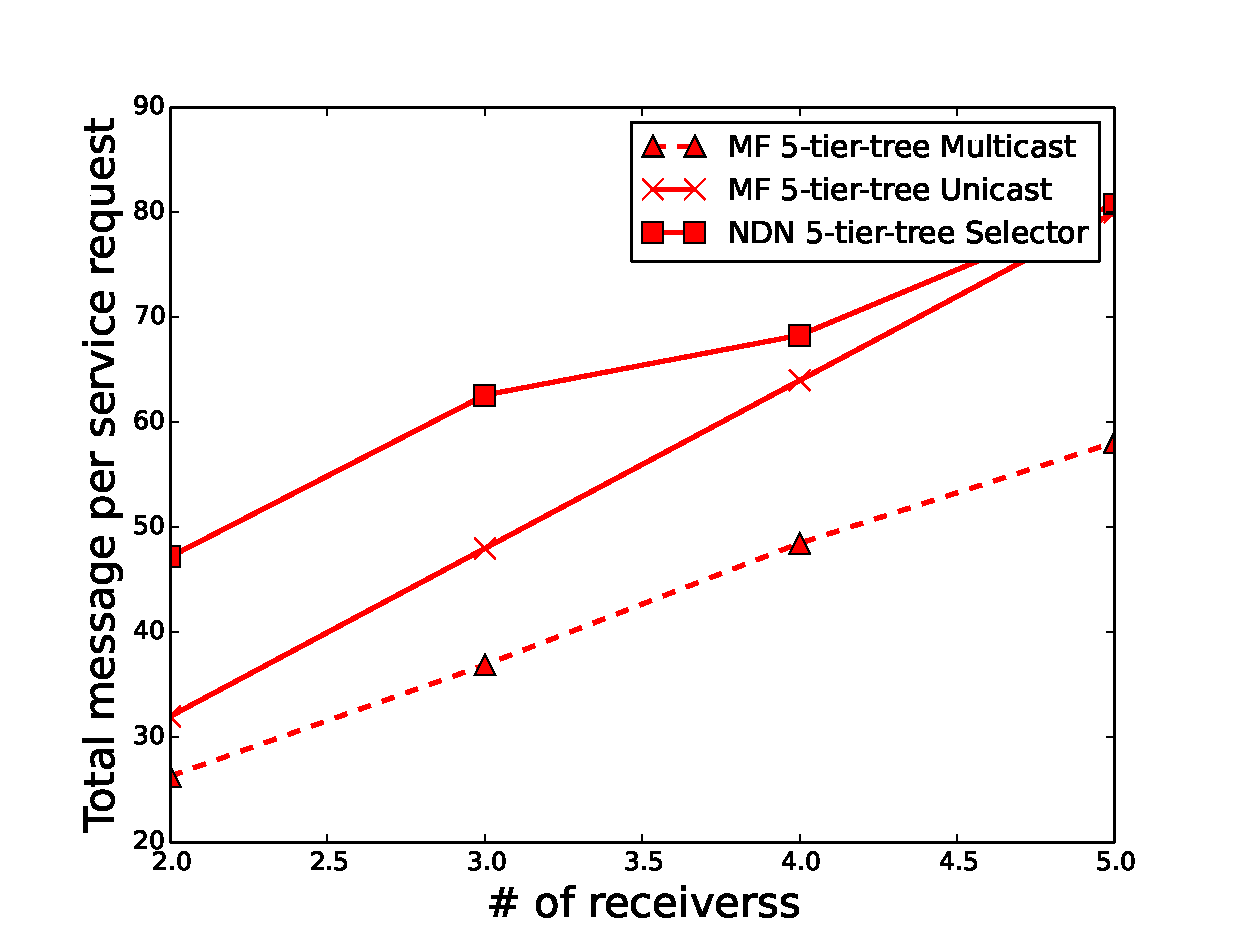
\includegraphics[width=\columnwidth]{figure/service_discovery_overhead.eps}
\caption{\label{fig:service_over}Overhead of service discovery in tree topology}
\end{figure}
\vspace{-1mm}
\begin{figure}
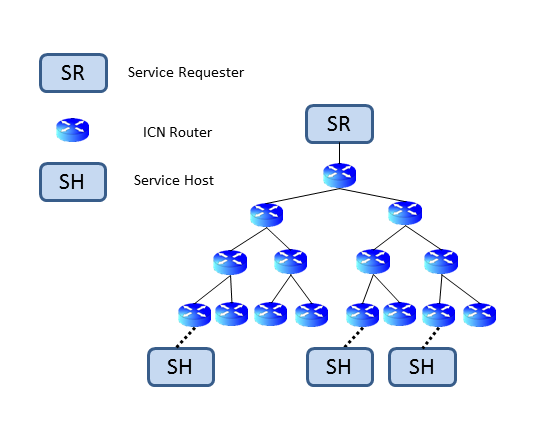
\includegraphics[width=\columnwidth]{figure/topology.png}
\caption{\label{fig:topology}Topology example for a 6-tier tree}
\end{figure}
\vspace{-1mm}
In this section, we investigate the efficiency of service discovery based on MF multicast, MF unicast and NDN interest selector. We have conducted detailed experiments in NS3-based MF simulator and ndnSIM.  MF network protocol is implemented over standard NS3 P2P module and the experiments are running in a tree-based topology. In MF multicast case, $Group GUID$ is used to identify a service at unknown location, i.e., service host (SH) can be located at any leaves of the tree while service requester (SR) attaches to the root of the tree. SR issues a request and the first router performs GNRS lookup for the $Group$-$GUID$. On receiving the service request message, the matched receivers will reply with an acknowledgement to the service requester via unicast. While in MF unicast case, we configure the SR to issue requests periodically and each matched SH will reply the request sequentially. In NDN selector experiment,  SR expresses Interest with name "/service", and corresponding full name is "/service/\{1,2,..., n\}". On receiving the response from one of the SHs, the SR appends the response's name to the exclusion list of a Interest and re-expresses a Interest with the same name. This operation will repeat until no response comes back. Figure~\ref{fig:service_over} shows the overhead in terms of total message per service discovery in tree topology that is shown in Figure~\ref{fig:topology}. In the 5-tier tree case, we observe that MF multicast introduces the least overhead among the three schemes, as it triggers only one GNRS lookup per request, and the routers only forwards request duplicates based on the next common hop(s). When the number of  SH increases to 5, NDN interest selector and MF unicast achieve similar performance. This is due to selector prevents both routers and SHs forwarding the discovered responses, which decreases the total response message. In MF unicast, total number of messages grows linearly as the number of SH increases. The result of another similar experiment but with a 6-tier tree demonstrates that NDN selector scheme encounters the highest overhead due to the impact of network scale increment on Interest broadcast.


%\subsection{Service Discovery}
%\subsection{Multi-source Retrieval}

